\chapter{Lösungskonzept}
    \label{chapter:SolutionConcept}
    Dieses Kapitel erläutert ein Lösungskonzept für die in Kapitel \ref{chapter:ProblemAnalysis} beschriebene Problemstellung.
    Zentrale Elemente dieser Lösung sind ein System zur automatischen Klassifizierung der Inhalte von Webseiten
    und eine \gls{dsl} zu dessen Instrumentierung.
    Das System heißt \gls{wccs}.

    \section{Klassen, Features und Selektoren}
    \section{Eine domänenspezifische Sprache zur Spezifikation von Klassen}
    \section{Klassifizierungsalgorithmus}
        \lstinputlisting[label=listing:classificationAlg,caption=Klassifizierungsalgorithmus]{../resources/classification.code}
    \section{Persistenz}
    \section{Visualisierung, Nachbesserung und Prüfung der Klassifikation}
    \section{Bereitstellung der Klassifikation zur Weiterverareitung}
    \section{Werkzeug zum Auffinden aller zu klassifizierenden Seiten}
    \section{Architektur}
        \label{section:Architecture}
        \subsection{Microservices Architekturen}

        % TODO Sollte WCCS component lieber WCCS service sein? Was mit DSL oder Crawler? Was wären das dann?
        \begin{figure}
            \centering
            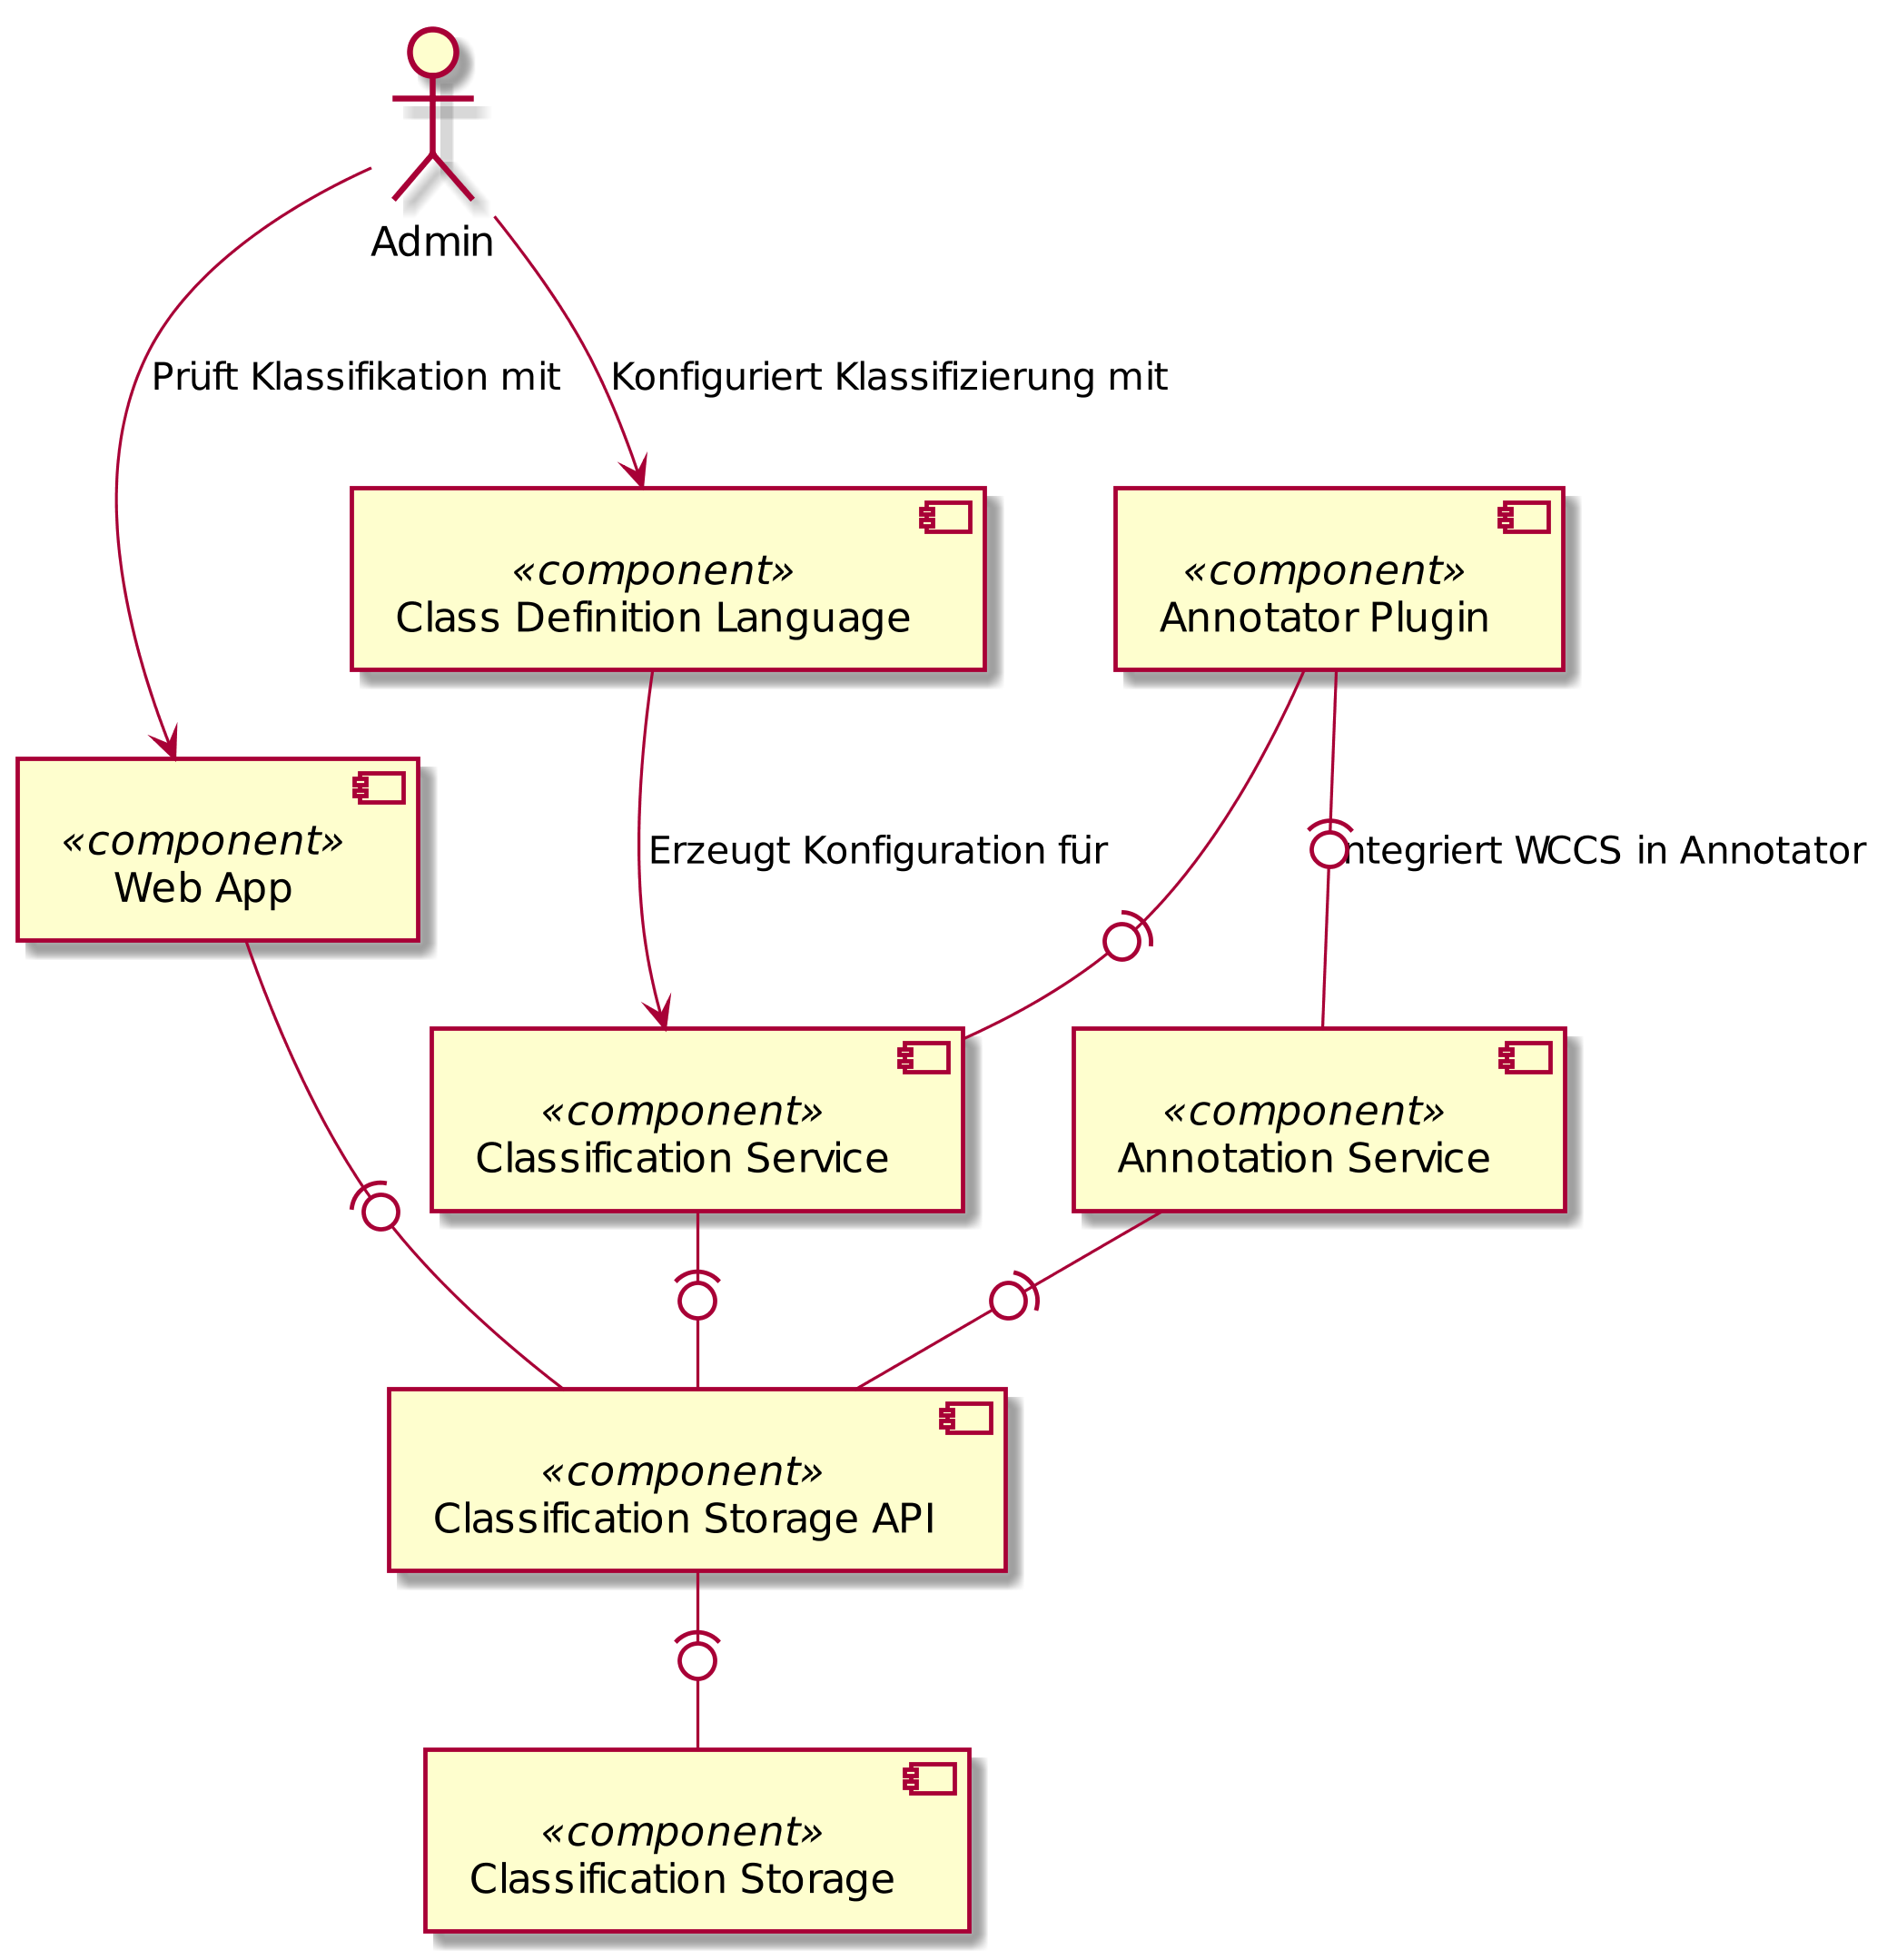
\includegraphics[width=\textwidth]{../resources/architecture/wccs_internal_architecture.png}
            \caption{Interne Architkektur von WCCS}
            \label{image:wccsInternalArchitecture}
        \end{figure}

        \begin{figure}
            \centering
            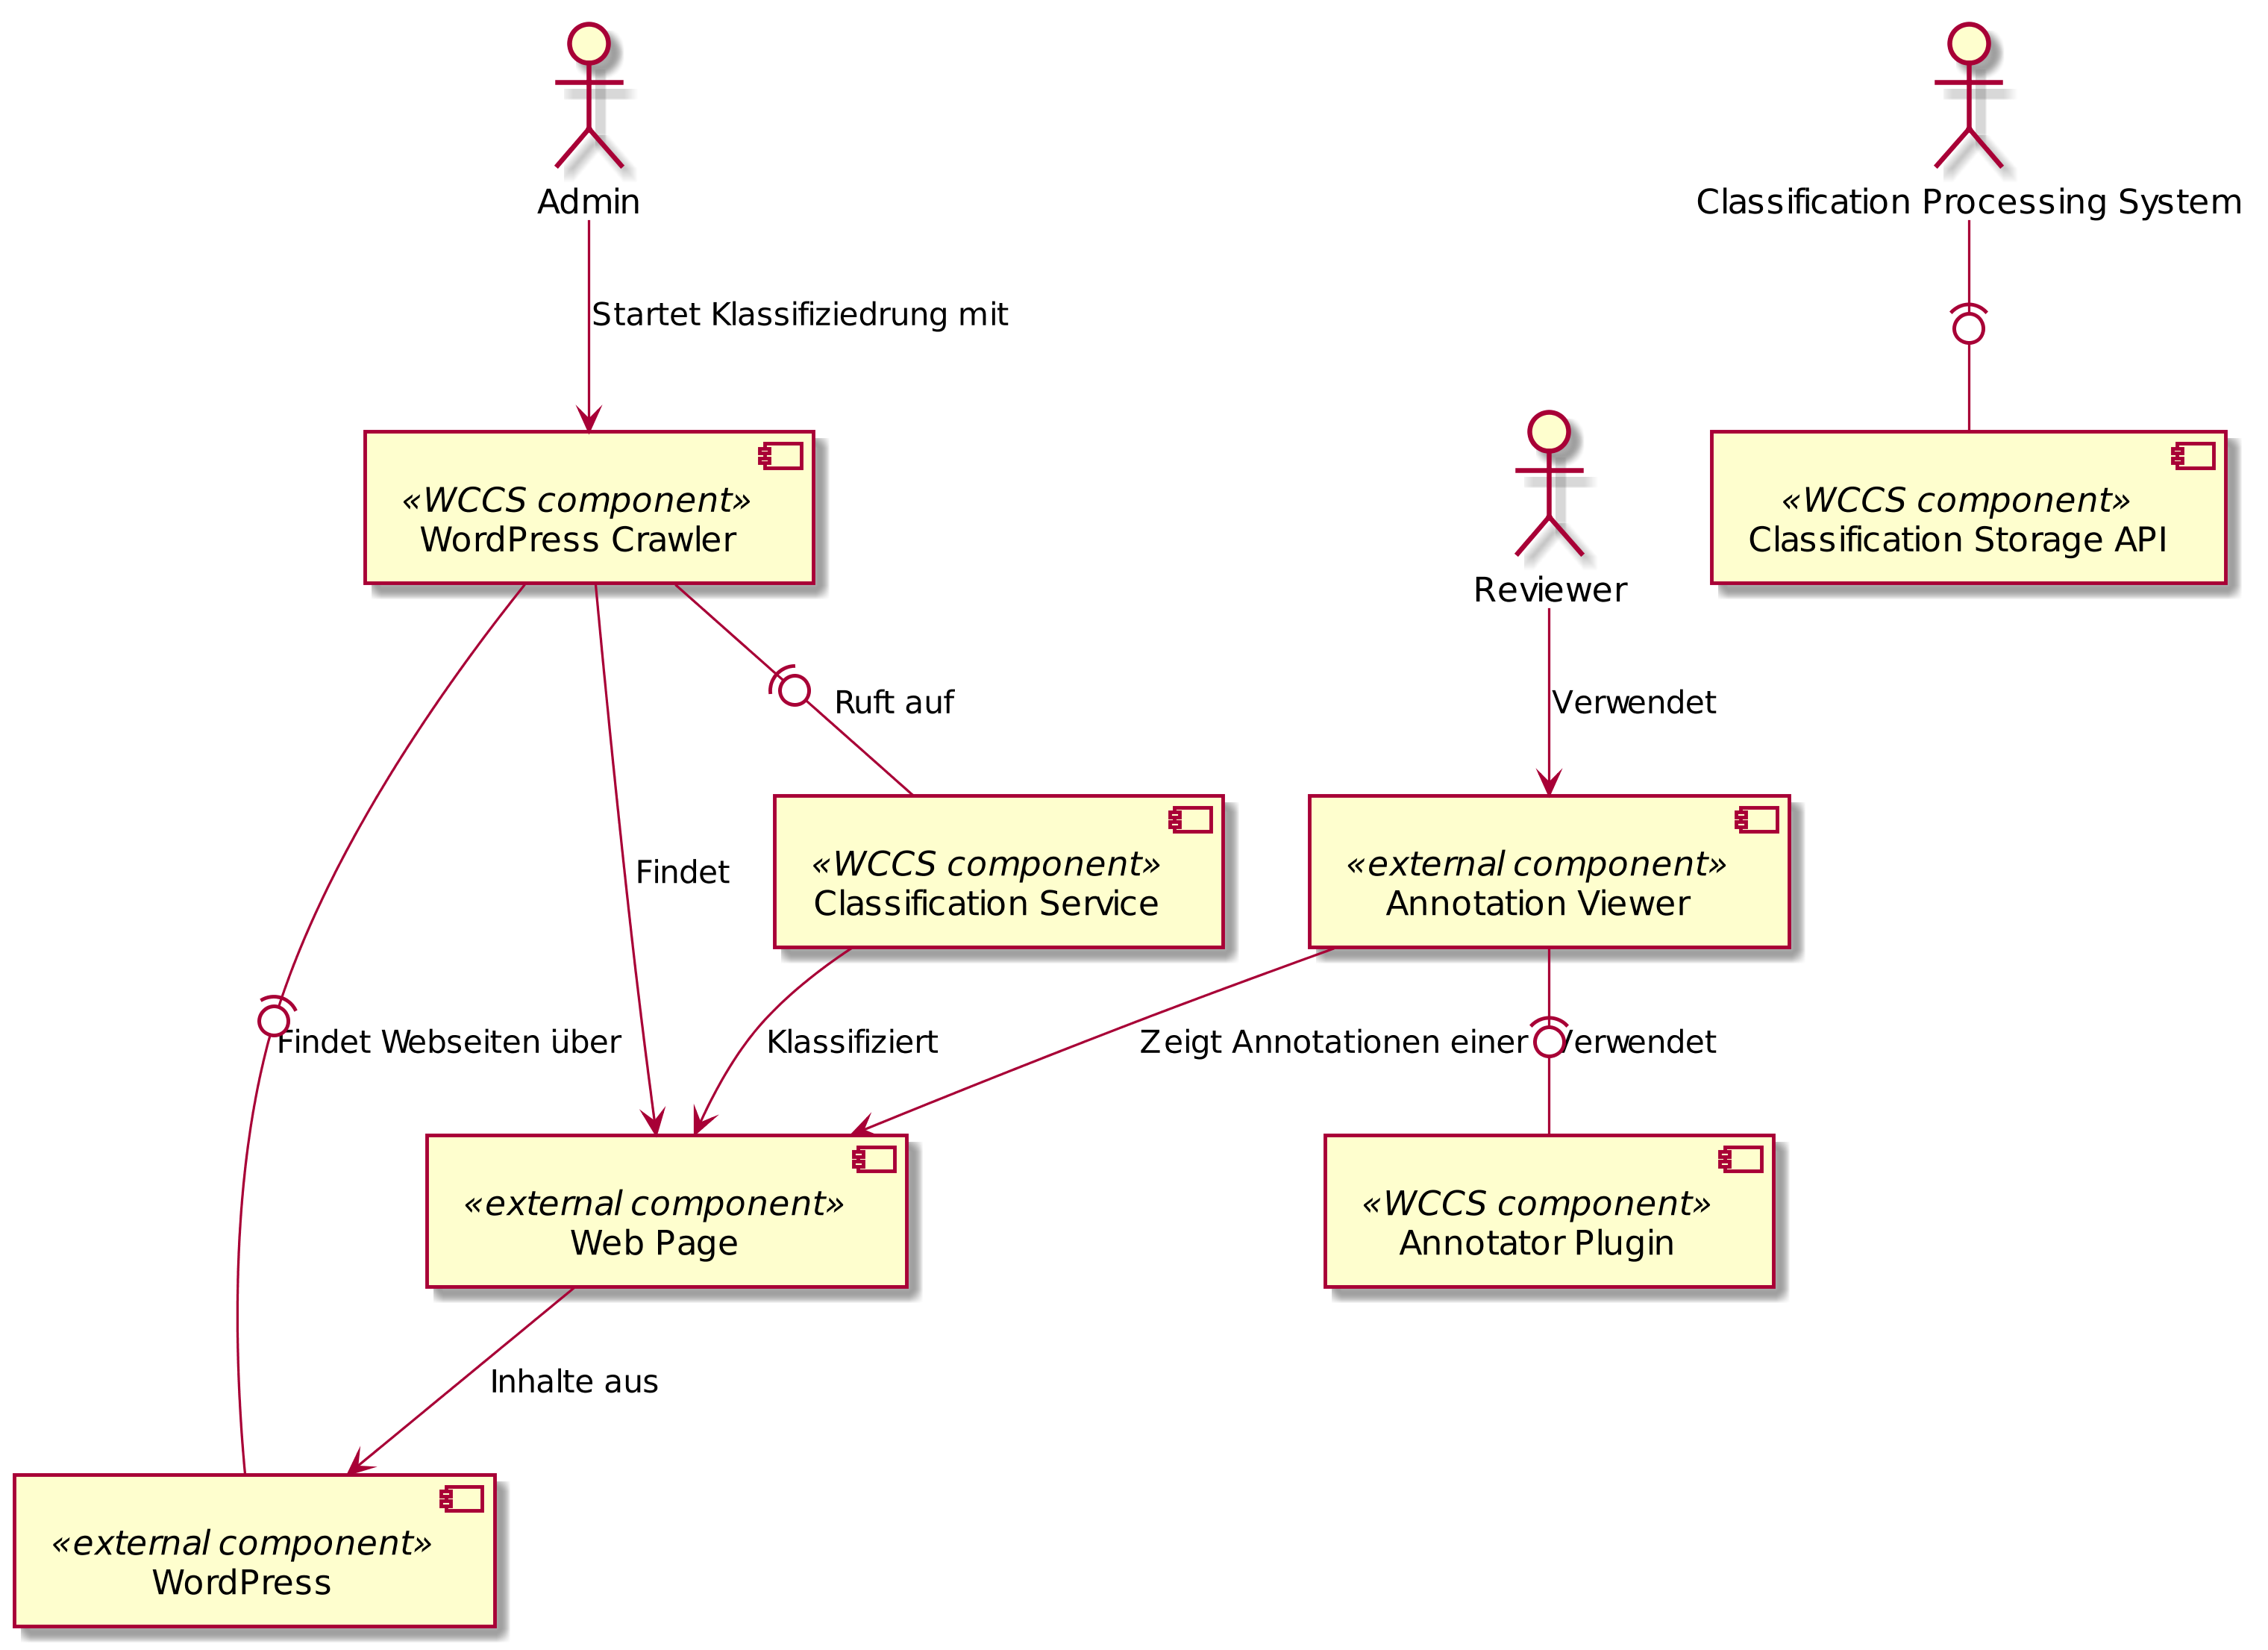
\includegraphics[width=\textwidth]{../resources/architecture/external_architecture.png}
            \caption{Externe Architkektur von WCCS}
            \label{image:wccsExternalArchitecture}
        \end{figure}